\documentclass[a4paper,10pt,twoside,twocolumn,bg=print]{dndbook} %a4, 10pt, book (idk why i did that...), 2 cols, dnd-themed
\usepackage[english]{babel} %language
\usepackage[utf8]{inputenc} %lovely utf-8
\usepackage{graphicx} %images
\usepackage{wrapfig} %images
\usepackage{tikz} %draw stuff
\usepackage{ifthen} %draw stuff
\usetikzlibrary{shapes,calc,fadings} %draw stuff
\usepackage{xspace} %usefull idk, allways import this stuff
\usepackage{setspace} %don't ask, kind of like it...
\usepackage{pgfplots}

\usepackage[singlelinecheck=false]{caption} %idk dndbook...
\usepackage{listings} %idk dndbook...
\usepackage{shortvrb} %not used yet...
\usepackage{stfloats} %idk dndbook
\usepackage{dirtytalk}
\usepackage{aurical} % nice font
\singlespacing
\makeatletter %because of titlepage and \HUGE

\@openrightfalse %no empty pages

\graphicspath{ {./images/} }

\def \license {GNU Free Documentation License}
\def \licensetext {Please consider and respect the copyleft of this license. The content of this document should be accessible to everyone. Everyone has the right to use the content of this document as he/she wishes, to modify it, to publish it modified (taking into account the copyleft) and to republish it without any changes (taking into account the copyleft).}
\author{Sven Hugi}%if you edit this document, add your name... <3
\def \accentcolor {PhbLightCyan}

%2 column layout hack...
\newcommand{\nextPage}{
	\newpage
	\hbox{}
	\newpage
}

\renewcommand{\maketitle}{
	\thispagestyle{empty}
	\onecolumn %fuck it
	\vspace*{5cm}
	\begin{center} \par\vspace{0.5cm}
		$\vspace*{2cm}$
		{\color{\accentcolor}\Huge \bf \Fontauri «Mystery of the Lythari» \par\vspace{0.5cm}}
		{\Large\Fontauri Puzzle-Oneshot for 4 level 10 players}
	\end{center}
	\twocolumn %reset shit
}\makeatother

\begin{document}
	\thispagestyle{empty}\setcounter{page}{0}\maketitle
	\onecolumn
	\section*{Credits}
	\makeatletter
	\vspace{.25cm}
	\textbf{Author:} \@author\linebreak
	\textbf{License:} \license\linebreak\linebreak
	\licensetext
	\makeatother
	\vfill
	\pagebreak
	\tableofcontents
	\vfill
	\pagebreak
	\section{Overview}
		\subsection{General informations}
			This oneshot is designed for 4 level 10 characters. If you want to play with less or more people and/or character on a different level, you should adjust the encounters.\linebreak
			The oneshot is designed for DnD 5e and will not work with earlier versions of the game.\linebreak
			There are no descriptions on how something locks in detail, you as the dm should explain it to the players as you imagine it.\linebreak
			Furthermore, the oneshot is designed to be fun and not to deliver particularly good encounters or extremely difficult puzzles.\linebreak
			And finally, if you want, you can customize the oneshot according to your own preferences. It can also be used to start a campaign.
		\subsection{Recommended optional rules}
		In this oneshot it's recommended to use some optional rules.
		\begin{itemize}
			\item Flanking
			\item Rule of Cool (really recommended)
			\item Feats
			\item Inspiration
			\item No XP (except you want to continue playing with this setting)
			\item Multiclassing
		\end{itemize}
	\vfill	
	\pagebreak
	\section{Story}
		In a nearby kingdom, the king was murdered by troops from haSyol. The son of the head wolf of a Lythari pack was there. When he took revenge on the king of haSyol, he realized that the troops from haSyol did not act without reason. If a war will break out, the pack could be in danger and if haSyol will lose, it will be a problem in anyway, because haSyol looks for small villages and settlements, the others only want to subjugate.\linebreak
		When the news came to the head wolf, he decided to get ancient magical weapons from a temple. These weapons were left there by them hundreds of years ago. They served in a previous war, when they helped the druids against a group of necromancers. The temple is well protected by traps and puzzles, so a team of the four best adventurers has been put together to retrieve the weapons. Now the four of you are gathered in front of the temple.\linebreak
		What do you want to do next?
	\section{Quest}
		Bring back the magic weapons from the temple.\linebreak
		The oneshot is over, if they leave the temple with the weapons
	\vfill
	\pagebreak
	\section{Maps}
		The default grid-size is 5 ft per square.
		\subsection{World map}
		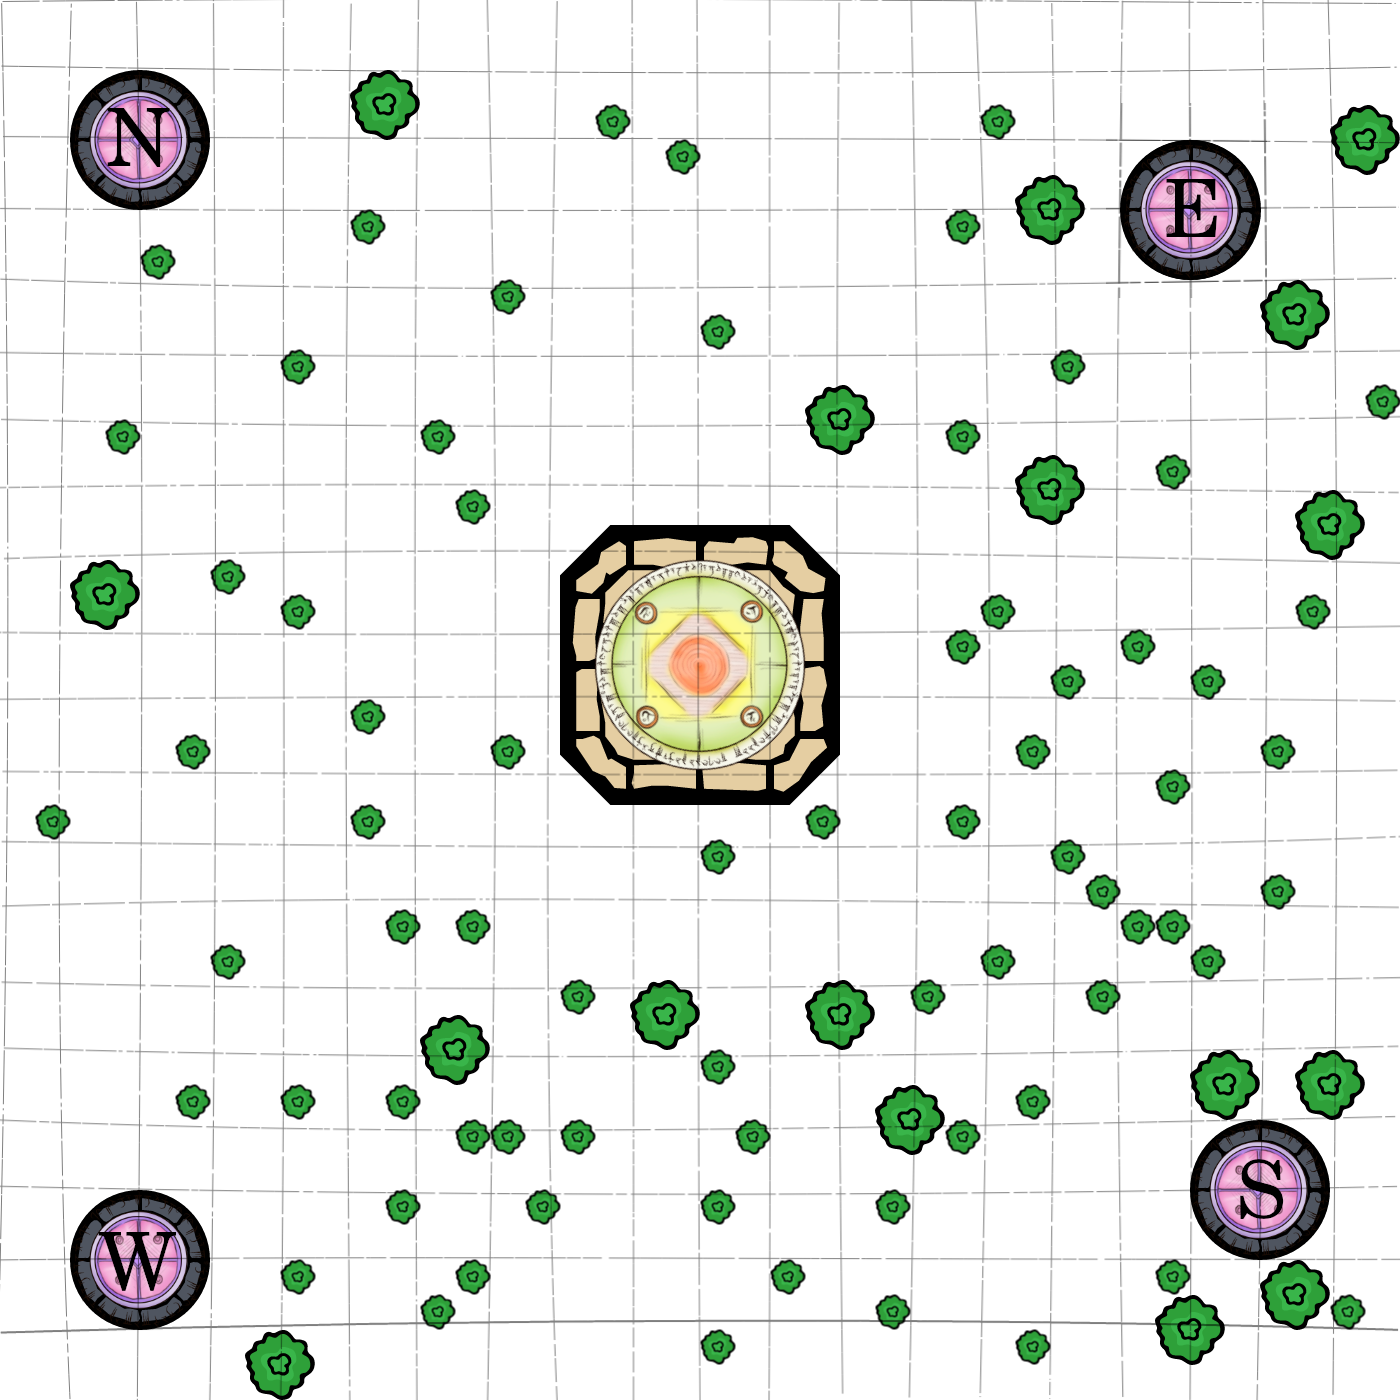
\includegraphics[width=\linewidth]{Map50Grid.png}
		\vspace*{4cm}\linebreak
		The map consists of a temple and four towers around it (one in each direction, north, east, south west). The towers around the temple each contain a crystal under the roof. This map uses a 50 ft grid.
		\vfill
		\pagebreak
		\subsection{Temple map}
		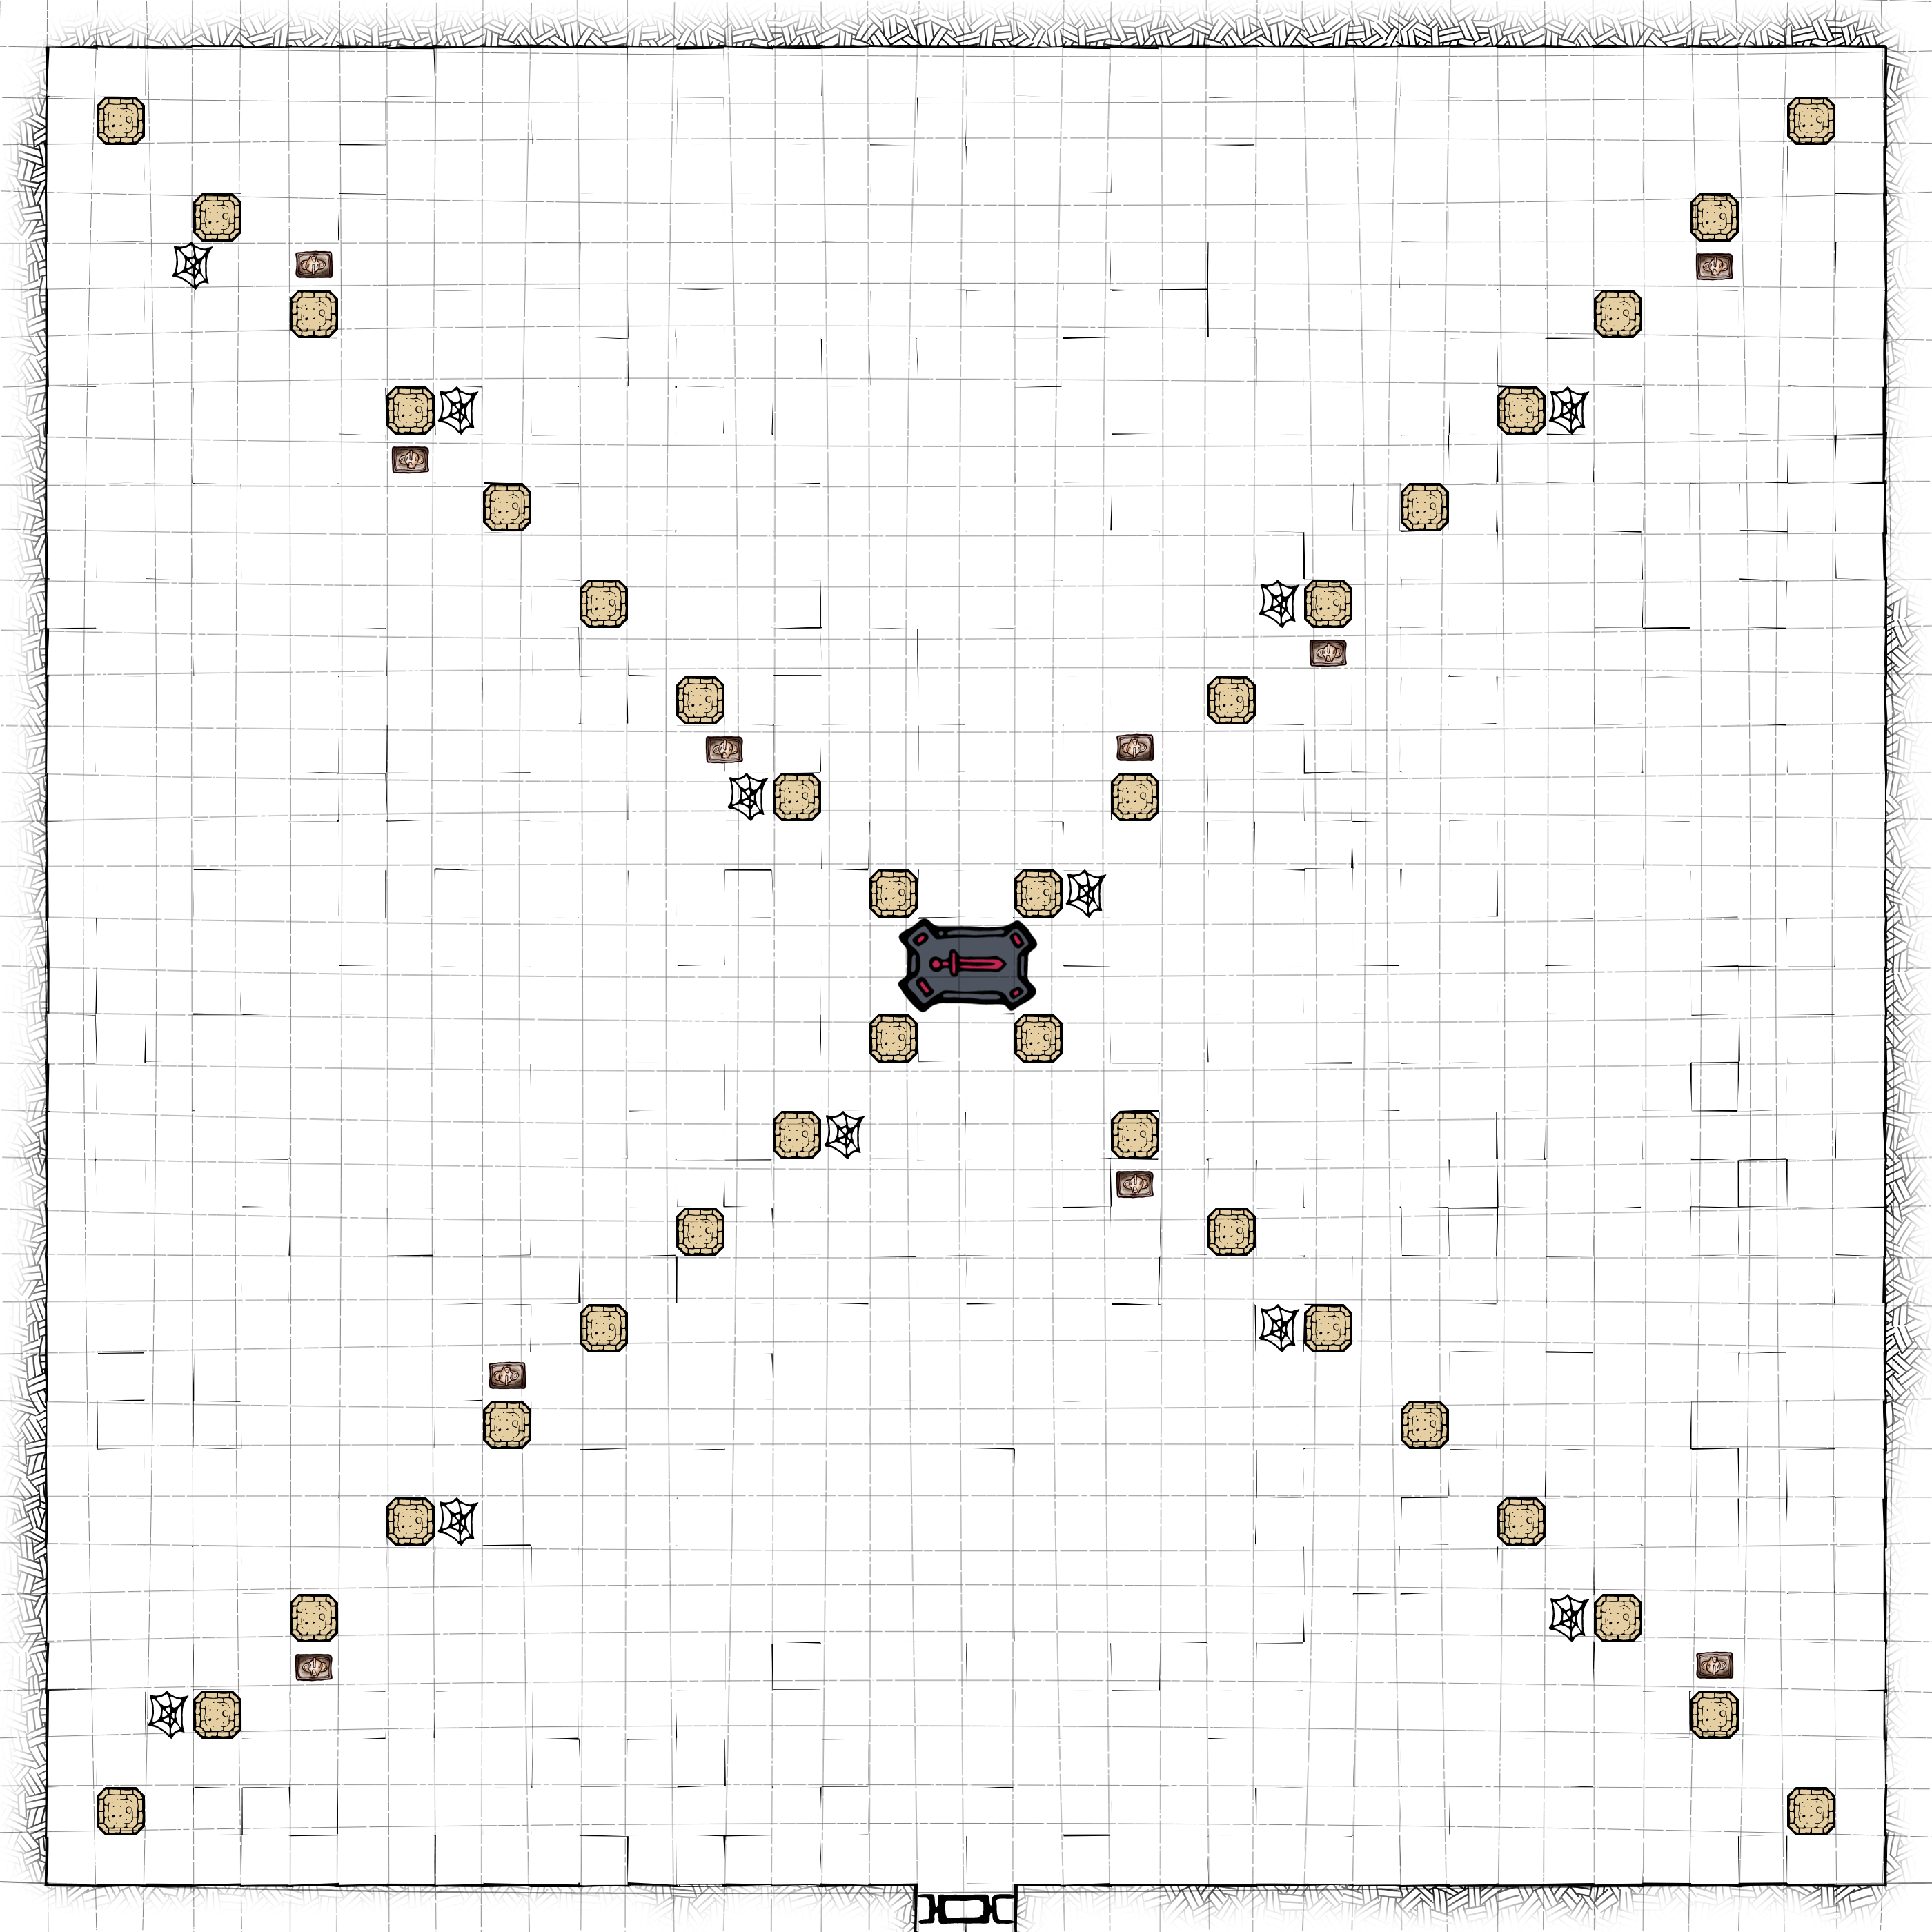
\includegraphics[width=\linewidth]{Temple.png}
		\vspace*{4cm}\linebreak
		The door at the temple opens as soon as all the crystals in the towers are activated. There are pillars across the hole temple. In the middle of the temple is an altar. Scattered around the temple are also some armors.
		\vfill
		\pagebreak
		\subsection{Tower 1 map}
		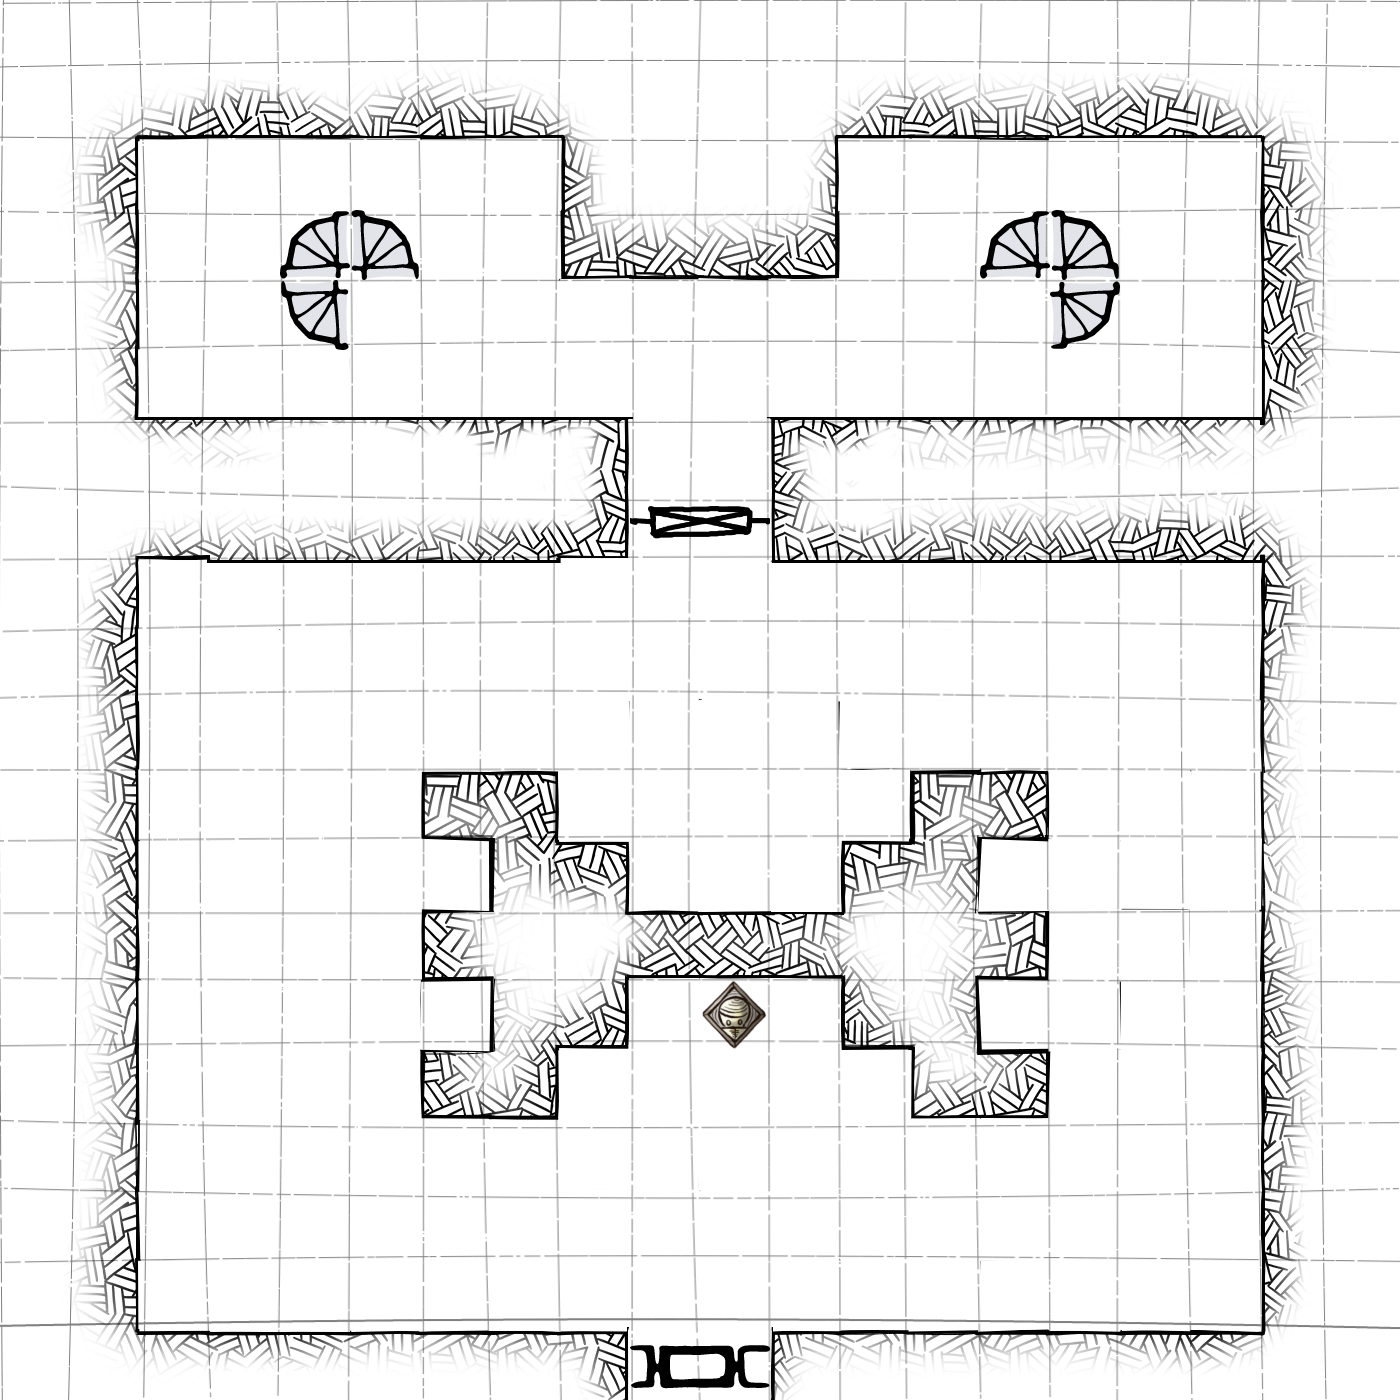
\includegraphics[width=\linewidth]{Tower1.png}
		\vspace*{4cm}\linebreak
		In the first tower (north) there is a locked door and a golem. Behind this door, there are two spiral staircases leading under the roof of the tower, there one of the crystals is located.
		\vfill
		\pagebreak
		\subsection{Tower 2 map}
		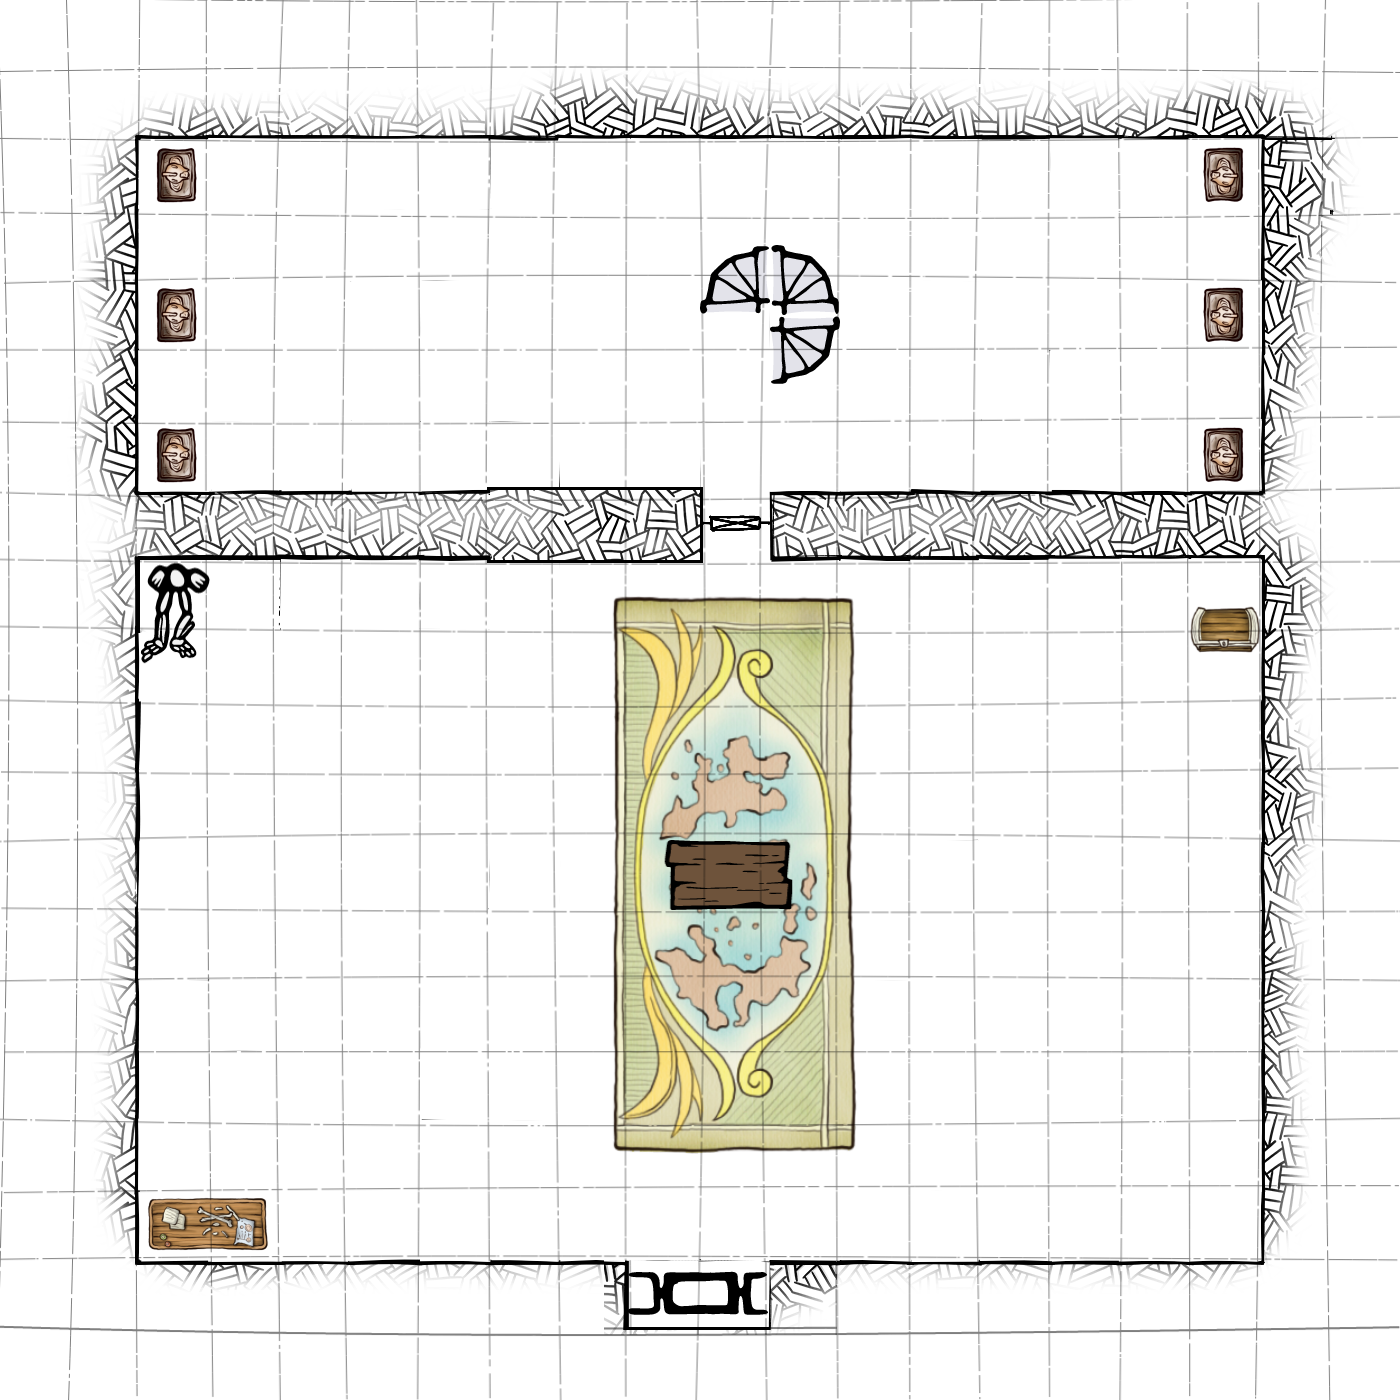
\includegraphics[width=\linewidth]{Tower2.png}
		\vspace*{4cm}\linebreak
		In the second tower (east) there is a table on a carpet. In one corner of the room there is a chest, in another a desk and in the third a skeleton. There is also a locked door. Behind it is a room with 6 armors and a spiral staircase that leads to the roof, where one of the crystals is located.
		\vfill
		\pagebreak
		\subsection{Tower 3 map}
		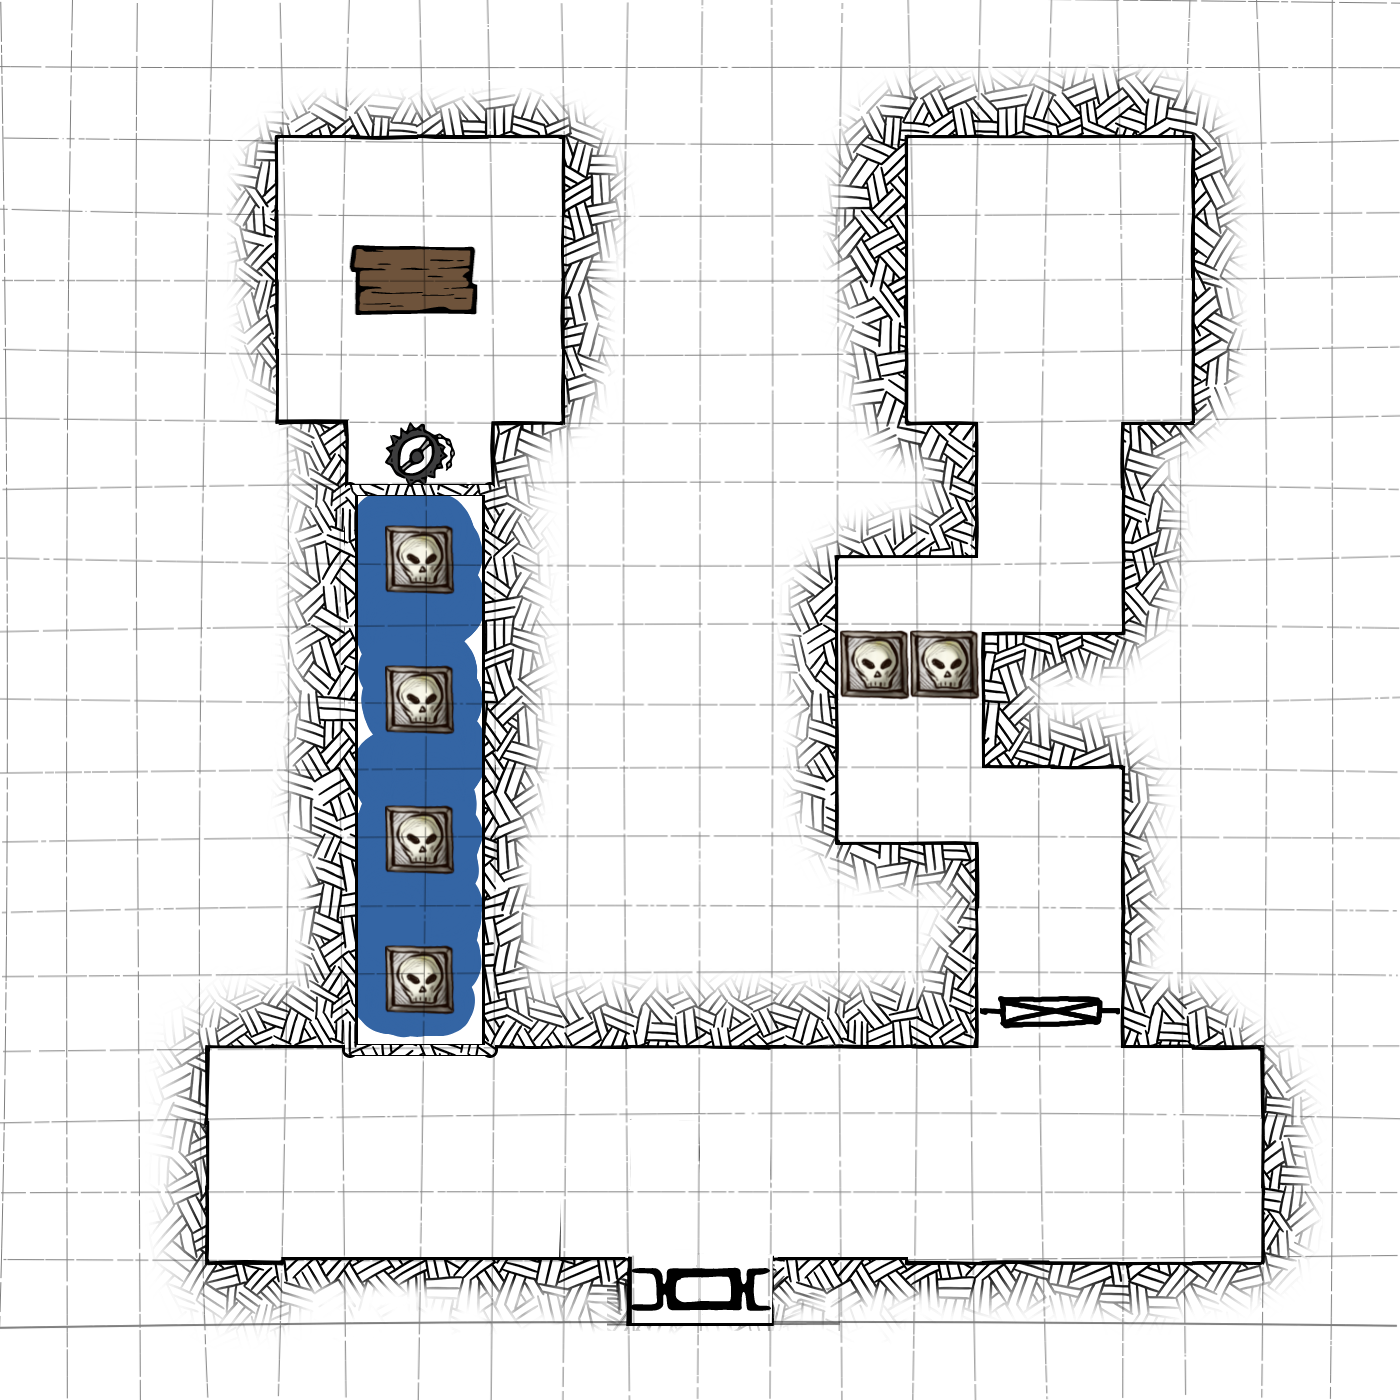
\includegraphics[width=\linewidth]{Tower3.png}
		\vspace*{4cm}\linebreak
		In the third tower (south) there is a small oblong room, leading to a pool and a locked door. Above the pool there are ropes and in the pool there are four giant octopuses. Behind the pool there is a table  with a key on it visible. Behind the closed door is a long corridor with two wolfs which leads to a small room with a teleporter. The teleporter leads under the roof, where one of the crystals is located.
		\vfill
		\pagebreak
		\subsection{Tower 4 map}
		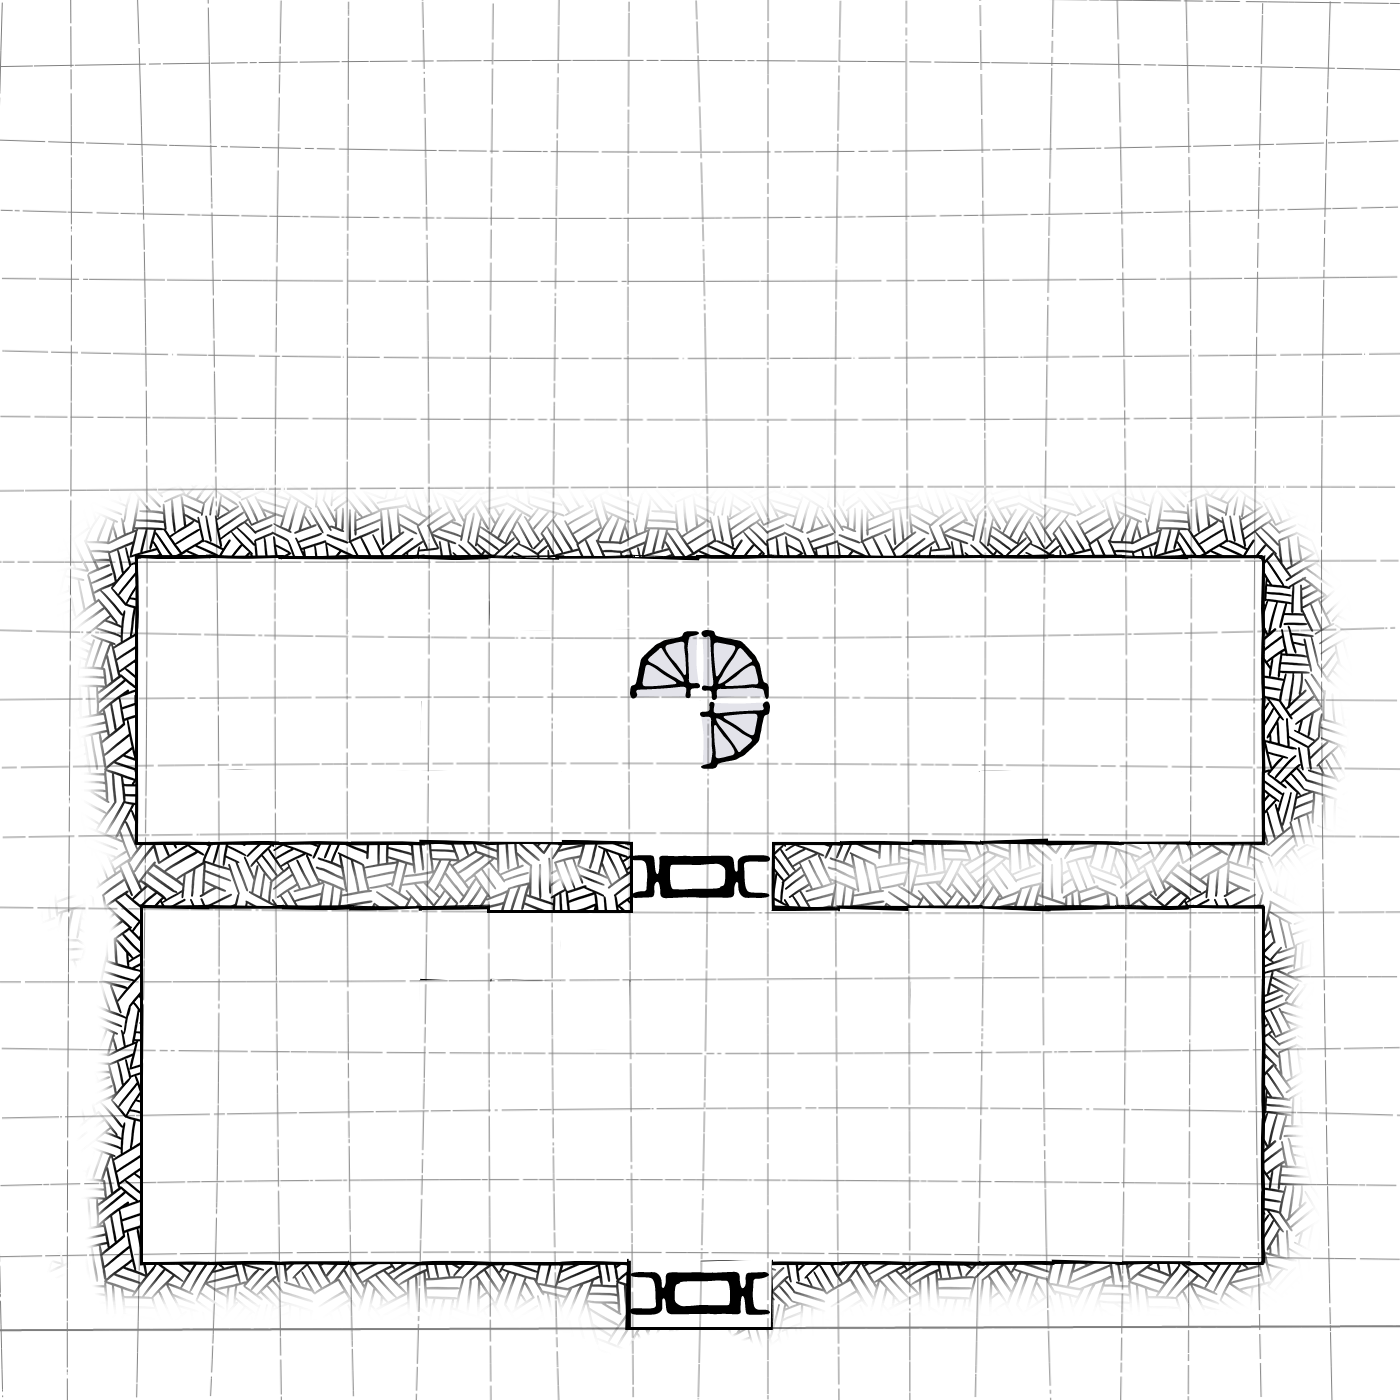
\includegraphics[width=\linewidth]{Tower4.png}
		\vspace*{4cm}\linebreak
		In the forth tower (west) there is a large empty room with a big mirror hanging on one wall. Behind the mirror is a other empty room with a spiral staircase leading under the roof, where one of the crystals is located.
		\vfill
		\pagebreak
	\section{Loot}
		\subsection{Temple}
			{\Large Altar}
				\DndItemHeader{Puncture Bow}{Martial Ranged Weapon, very rare}
					1d8 Piercing, Ammunition (range 150/600), two-handed, 2 lb\linebreak
					If a creature is hit by this bow and there is another creature in the same line within 60 feet, that creature is also attacked. This can repeat up to 5 times, with each time the damage increasing by 1d6.
				\DndItemHeader{Vicious Longbow}{Martial Ranged Weapon, rare}
					1d8 Piercing, Ammunition (range 150/600), heavy, two-handed, 2 lb\linebreak
					When you roll a 20 on your attack roll with this Longbow, the target takes an extra 7 piercing damage.
				\DndItemHeader{Mistyblade}{Martial Weapon, very rare}
					1d10 Slashing, Versatile (1d12), 3 lb\linebreak
					When you hit a creature with this longsword you can use your movement in form of the misty step spell. You also gain a +2  bonus to attack and damage rolls made with this weapon.
				\DndItemHeader{Sun Blade}{Martial Weapon, rare}
					This item appears to be a longsword hilt. While grasping the hilt, you can use a bonus action to cause a blade of pure radiance to spring into existence, or make the blade disappear. While the blade exists, this magic longsword has the finesse property. If you are proficient with shortswords or longswords, you are proficient with the sun blade.\linebreak
					You gain a +2 bonus to attack and damage rolls made with this weapon, which deals radiant damage instead of slashing damage. When you hit an undead with it, that target takes an extra 1d8 radiant damage.\linebreak
					The sword's luminous blade emits bright light in a 15-foot radius and dim light for an additional 15 feet. The light is sunlight. While the blade persists, you can use an action to expand or reduce its radius of bright and dim light by 5 feet each, to a maximum of 30 feet each or a minimum of 10 feet each.\linebreak
					Proficiency with a longsword allows you to add your proficiency bonus to the attack roll for any attack you make with it.
		\subsection{Tower 1}
			There is no loot in the first tower.
			\vfill\pagebreak
		\subsection{Tower 2}
			{\Large Table}
				\begin{itemize}
					\item Gem
				\end{itemize}
			{\Large Chest}
				\begin{itemize}
					\item 5 GP
					\item Shield
					\item Dagger
					\item Old key
					\item Bag with rotten herbs
					\item Gold ring (arcane focus)
				\end{itemize}
			{\Large Desk}
				\begin{itemize}
					\item 1 SP
					\item Ink pen
					\item Ink bottle
					\item Old book with unreadable writing (gibberish)
					\item Clay pitcher (for the Puzzel in Tower 4)
				\end{itemize}
			{\Large Under Carpet}
				\begin{itemize}
					\item 4 CP
					\item 5 Mirrors
					\item Small green Stone
					\item Old rusty key
					\item Pieces of clay
				\end{itemize}
			{\Large Skelet}
				\begin{itemize}
					\item Bones
					\item Silver ring
				\end{itemize}
			{\Large Armor (each)}
				\begin{itemize}
					\item Longsword
				\end{itemize}
		\subsection{Tower 3}
			{\Large Table}
				\begin{itemize}
					\item Key for the door in the same room
				\end{itemize}
		\subsection{Tower 4}
			There is no loot in the fourth tower.
	\vfill
	\pagebreak
	\section{Traps}
		\DndItemHeader{Improved Bear Trap}{Simple Trap}
		A bear trap resembles a set of iron jaws that springs shut when stepped on, clamping down on a creature's leg. The trap is spiked in the ground, leving the victims immobilized.\\
		\textbf{Trigger.} A creature that steps on the bear trap triggers it.\\
		\textbf{Effect.} The trap makes an attack against the triggering creature. The attack has a +10 attack bonus and deals \DndDice{2d10} piercing damage on a hit. The attack can't gain advantage or disadvantage. A creature hit by the trap has its speed reduced to 0. It can't move until it breaks free of the trap, which requires a successfull DC 18 Strenght check by the creature or another adjacent to the trap.\\
		\textbf{Countermeasures.} A successful DC 12 Wisdom (Perception) check reveals the trap. A Successful DC 15 Dexterity check using thievens'tools disables it. A Character can step over the trap with a successful DC 16 Dexterity check.
	\vfill
	\pagebreak
	\section{Puzzles}
		\subsection{Temple Door Puzzle}
			Temple\linebreak
			To open the door of the temple, you need to activate four crystals located under the roofs of the four towers around the temple. Activation is possible with either a spell or cantrip that produces light or radiant damage, or if no character can handle spells, with a torch. On the door of the temple there are four gems, with the letters N, E, S and W in it, those gems glow, when the crystal in the corresponding tower is activated. 
		\subsection{Golem Encounter}
			Tower 1\linebreak
			After killing the golem, the door opens.
		\subsection{Gem Puzzle}
			Tower 2\linebreak
			The puzzle consists of an oak table on which a gemstone is placed, there is also a carpet under the oak table. On the table is a writing: \say{A cross formed without breaking from the one gem, shall open the door. Infinite power it stands under the oak.} The solution here is to bring out four mirrors from under the carpet (Infinite power under the oak). If you place two mirrors opposite each other with the gemstone in the middle, it reflects infinitely.If you repeat the process with a second pair of mirrors, you can use the reflection to form a cross if you look at it at the right angle. That fulfills the condition. This puzzel is here quite clearly like a curse prescribed.
		\subsection{Pool Puzzle}
			Tower 3\linebreak
			The puzzle consists of a pool with four giant octopuses. Above them are ropes, from which you can swing back and forth (DC 15 Athletics or Acrobatics). At the end is a improved bear trap. While you are swinging back and forth, you get attacked by the octopuses (opportunity attack $\rightarrow$ grappled on a hit). The goal is to get the key on the table to open the next door. In itself there is no real solution to this puzzle, just get the key.
		\subsection{Wolf}
			Tower 3\linebreak
			To avoid the encounter with the wolf, a lythari must be in wolf form or one of the characters must have a wolf familiar with them. This must happen before the fight.
		\subsection{Mirror Puzzle}
			Tower 4\linebreak
			The door that prevents you from going further is a mirror. In the reflection in this mirror you can see a clay pitcher, which is not visible on your side. The solution is to either find the clay pitcher and place it so that it matches the reflection, or to create an illusion that matches it. After that the mirror shatters into pieces. The mirror cannot be broken in any other way or magically bypassed.
	\vfill
	\pagebreak
	\section{Encounter}
		\subsection{Animated Armor I}
			Temple\linebreak
			When the weapons are taken from the altar, the 10 armors, which are scattered across the temple, come to life and chase the characters. They can fight or just leave.
		\subsection{Golem}
			Tower 1\linebreak
			The golem starts attacking the players, as soon as they enter the room. There is only one golem and he is located a few feet in front of the middle wall facing to the entrance.
		\subsection{Animated Armor II}
			Tower 2\linebreak
			If a player is in a 20 ft radius of one of the armors, the whole site (3 armors) attacks. In total there are six armors split to two groups, standing on the wall in the room with the staircase.
		\subsection{Giant Octopus}
			Tower 3\linebreak
			The four giant octopuses attack, as soon as someone wants to cross the small pool where they are in. In total there are four giant octopuses.
		\subsection{Wolfs}
			Tower 3\linebreak
			The Wolfs start to attack the party, as soon as they can see them. Except a lythari is in wolf form or one of the characters has a wolf familiar with them. In total there are two wolfs and they are located in the corridor behind the door.
	\vfill
	\pagebreak
	\section{Monster Stats}
		\begin{DndMonster}{Golem}
		\DndMonsterType{Large construct, unaligned}
		\DndMonsterBasics[
		armor-class = {17 (natural armor)},
		hit-points  = {\DndDice{17d10 + 85}},
		speed       = {30 ft.},
		]
		\DndMonsterAbilityScores[
		str = 22,
		dex = 9,
		con = 20,
		int = 3,
		wis = 14,
		cha = 1,
		]
		\DndMonsterDetails[
		damageimmunities = {poision, psychic},
		damageresistances = {bludgeoning, piercing, and slashing from nonmagical attacks},
		conditionimmunities = {charmed, exhaustion, frightened, paralyzed, petrified, poisoned},
		senses = {Darkvision 120ft., passive Perception 12},
		languages = {understands Elvish, but can't speak},
		challenge = 10,
		]
		\DndMonsterAction{Immutable Form}
		The golem is immune to any spell or effect that would alter its form.
		\DndMonsterAction{Magic Resistance}
		The golem has advantage on saving throws against spells and other magical effects.
		\DndMonsterAction{Magic Weapons}
		The golem's weapon attacks are magical.
		
		\DndMonsterSection{Actions}
		\DndMonsterAction{Multiattack}
		The golem makes two slam attacks
		%\DndMonsterMelee calls \DndMonsterAttack with the melee option
		\DndMonsterMelee[
		name=Slam,
		mod=+10,
		reach=5,
		targets=one target,
		dmg=\DndDice{3d8+6},
		dmg-type=bludgeoning,
		%plus-dmg=\DndDice{2d6},
		%plus-dmg-type=fire,
		%or-dmg=\DndDice{1d10+1},
		%or-dmg-when=if used with two hands,
		%extra=,
		]
		\DndMonsterMelee[
		name=Double slam (Recharge 5-6),
		mod=+14,
		reach=5,
		targets=one target,
		dmg=\DndDice{6d10+6},
		dmg-type=bludgeoning,
		%plus-dmg=\DndDice{2d6},
		%plus-dmg-type=fire,
		%or-dmg=\DndDice{1d10+1},
		%or-dmg-when=if used with two hands,
		%extra=,
		]
	\end{DndMonster}
	Drops: nothing
	\begin{DndMonster}{Wolf}
		\DndMonsterType{Medium beast, unaligned}
		\DndMonsterBasics[
		armor-class = {15 (natural armor)},
		hit-points  = {\DndDice{6d8 + 12}},
		speed       = {50 ft.},
		]
		\DndMonsterAbilityScores[
		str = 12,
		dex = 18,
		con = 14,
		int = 6,
		wis = 14,
		cha = 10,
		]
		\DndMonsterDetails[
		skills = {Perception +5, Stealth +7},
		senses = {Darkvision 60ft., passive Perception 12},
		languages = {-},
		challenge = 2,
		]
		\DndMonsterAction{Keen Hearing and Smell}
		The wolf has advantage on Wisdom (Percetion) checks that rely on hearing or smell.
		\DndMonsterAction{Pack Tactics}
		The wolf has advantage on attack rolls against a creature if at least one of the wolf's allies is within 5 feet of the creature and the ally isn't incapacitated.
		
		\DndMonsterSection{Actions}
		\DndMonsterAction{Multiattack}
		The wolf makes two bite attacks
		%\DndMonsterMelee calls \DndMonsterAttack with the melee option
		\DndMonsterMelee[
		name=Bite,
		mod=+7,
		%reach=5,
		targets=one target,
		dmg=\DndDice{1d8+4},
		dmg-type=piercing,
		%plus-dmg=\DndDice{2d6},
		%plus-dmg-type=fire,
		%or-dmg=\DndDice{1d10+1},
		%or-dmg-when=if used with two hands,
		%extra=,
		]
	\end{DndMonster}
	Drops: nothing
	\vfill
	\pagebreak
	\begin{DndMonster}{Animated Armor}
		\DndMonsterType{Medium construct, unaligned}
		\DndMonsterBasics[
		armor-class = {18 (natural armor)},
		hit-points  = {\DndDice{6d8 + 6}},
		speed       = {25 ft.},
		]
		\DndMonsterAbilityScores[
		str = 14,
		dex = 11,
		con = 13,
		int = 1,
		wis = 3,
		cha = 1,
		]
		\DndMonsterDetails[
		conditionimmunities = {blinded, charmed, deafend, exhaustion, frightend, paralyzed, petrified, poisoned},
		damageimmunities = {poison, psychic},
		senses = {Blindsight 60ft. (blinded beyond this radius), passive Perception 6},
		languages = {-},
		challenge = 1,
		]
		\DndMonsterAction{Antimagic Susceptibility}
		The armor is incapacitated while in the area of an antimagic field. If targeted by dispel magic, the armor must succeed on a Constitution saving throw against the caster's spell save DC or fall unconcious for 1 minute.
		\DndMonsterAction{False Appearance}
		While the armor remains motionless, it is indistinguishable from a normal suit of armor.
		
		\DndMonsterSection{Actions}
		\DndMonsterAction{Multiattack}
		The armor makes two melee attacks
		%\DndMonsterMelee calls \DndMonsterAttack with the melee option
		\DndMonsterMelee[
		name=Longsword,
		mod=+4,
		reach=5,
		targets=one target,
		dmg=\DndDice{1d8+2},
		dmg-type=slashing,
		%plus-dmg=\DndDice{2d6},
		%plus-dmg-type=fire,
		%or-dmg=\DndDice{1d10+1},
		%or-dmg-when=if used with two hands,
		%extra=,
		]
	\end{DndMonster}
	Drops: Longsword (Martial Melee Weapon, 1d8 Slashing, Versatile (1d10), 3 lb)
	\begin{DndMonster}{Giant Octopus}
		\DndMonsterType{Large beast, unaligned}
		\DndMonsterBasics[
		armor-class = {11},
		hit-points  = {\DndDice{10d10 + 10}},
		speed       = {10 ft., swim 60ft},
		]
		\DndMonsterAbilityScores[
		str = 18,
		dex = 13,
		con = 13,
		int = 6,
		wis = 12,
		cha = 4,
		]
		\DndMonsterDetails[
		skills = {Perception +5, Stealth +5},
		senses = {Darkvision 60ft., passive Perception 15},
		languages = {-},
		challenge = 2,
		]	
		\DndMonsterAction{Hold Breath}
		While out of water, the octopus can hold its breath for 1 hour.
		\DndMonsterAction{Underwater Camouflage}
		The octopus has advantage on Dexterity (Stealth) checks made while underwater.
		\DndMonsterAction{Water Breathing}
		The Octopus can breathe only underwater.
		
		\DndMonsterSection{Actions}
		%\DndMonsterMelee calls \DndMonsterAttack with the melee option
		\DndMonsterMelee[
		name=Tentacles,
		mod=+6,
		reach=15,
		targets=one target,
		dmg=\DndDice{2d8+4},
		dmg-type=bludgeoning,
		%plus-dmg=\DndDice{2d6},
		%plus-dmg-type=fire,
		%or-dmg=\DndDice{1d10+1},
		%or-dmg-when=if used with two hands,
		extra={If the target is a creature, it is grappled (escape DC 17). Until this grapple ends, the target is restrained, and the octopu can't use its tentacles on anoter target},
		]
		\DndMonsterAction{Ink Cloud (Recharges after a Short or Long Rest)}
		A 20-foot-radius cloud of ink extends all around the octopus if it is underwater. The are is heavily obscured for 1 minute, although a significant current can disperse the ink. After releasing the ink, the octopus can use the Dash action as a bonus action.
	\end{DndMonster}
	Drops: nothing
	\vfill
\end{document}